% Charlotte Geiger - Manuel Lippert - Leonard Schatt
% Physikalisches Praktikum

% 3.Kapitel  Protokoll

% Variables
\def\skalierung{0.65}

\chapter{Setup and Methods}
\label{chap:methods}
\section{Setup}\label{sec:setup}
In the following section, the setup for the lightsheet microscope is explained. \\
The laser is decoupled from another experiment. Its power is controlled by a computer program via the current $I_L$. Using mirrors, the beam is deflected to two lenses forming a telescope which widens it. The lightsheet is created using a cylinder lense and an excitation objective. The latter is inside the SPIM chamber filled with UV water focussing on the probe. Motion of the probe is possible via a motorized mount. The detection of the fluorescence is provided by a detection objective which also is inside the chamber. A mask and a filter are used to block any unwanted scattered light. A tubus lense focusses the light in a DFC camera. An overview over the setup is shown in fig.~\ref{fig:setup}.

\begin{figure}[ht]
    \centering
    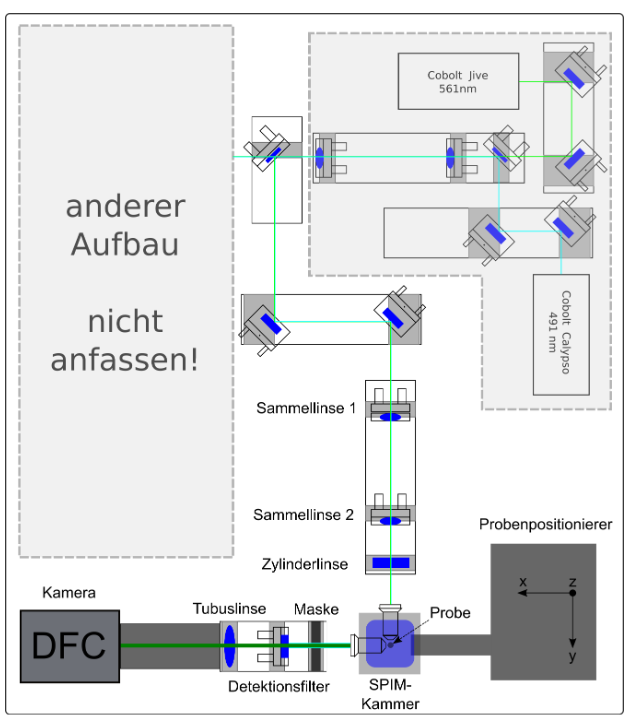
\includegraphics[width = \textwidth]{Bilder/Setup/setup.png}
    \caption{Overview of the used setup. For details see main text. Figure from~\cite{Struntz.2017}.}
    \label{fig:setup}
\end{figure}



\section{Methods}\label{sec:methods}
\subsection*{Characterization of the lightsheet}

For the characterization of the lightsheet no sample was used, the SPIM chamber was just filled with UV water. For the control of the camera and mount the program Micro-Manager was used. As no fluorescent particles were present, the filter was taken out. First, the lightsheet had to be found in the chamber. Then, it was measured for three different widths of the laser beam using no pinhole, a half opened pinhole and a closed pinhole. For each, 100 images were taken with a temporal distance of \SI{1}{\milli\second}, an exposure time of \SI{40}{\milli\second}, gain set to maximum and a laser power corresponding to \SI{2.6}{\ampere}. For the closed pinhole the laser current had to be increased to \SI{2.7}{\ampere} due to low intensity. 

\subsection*{Characterization of the setup using a bead probe}
For the characterization of the setup a bead probe was made. Therefore, fluorescent polystyrene beads with a diameter of \SI{200}{\nano\meter} were dilluted in UV water 1:1000. The solution was put in an ultrasonic bath to reduce possible agglomerates. The bead solution then was vortexed with a \SI{2}{\percent}wt agarose solution. The mixture was pipetted in a syringe with the top cut off. The syringe was placed in the fridge to accelerate the gelation. After that, the cylindrical sample could be easily ejected partly from the syringe and mounted in the SPIM chamber.\\
The objectives were refocussed, the filter set back in and the pinhole taken out. First, four sites of the probe were measured: one close to the detection objective (1), one in the center of the probe (2), one close to the illumination objective (3) and one along the curvature between site (1) and site (3) (4). The sites are displayed in fig.~\ref{fig:sites}. For each measurement a z-stack of 200 images was taken with a distance between the images of \SI{200}{\nano\meter}. The exposure time was set to \SI{25}{\milli\second}, the gain to \num{1} and the laser current to \SI{2.5}{\ampere}. As position (1) showed the most promising resolution, z-stacks of the same properties were taken there using a half opened pinhole ($I_L=$\SI{2.4}{\ampere}) and with a closed pinhole ($I_L=$\SI{2.7}{\ampere}).

\begin{figure}[ht]
    \centering
    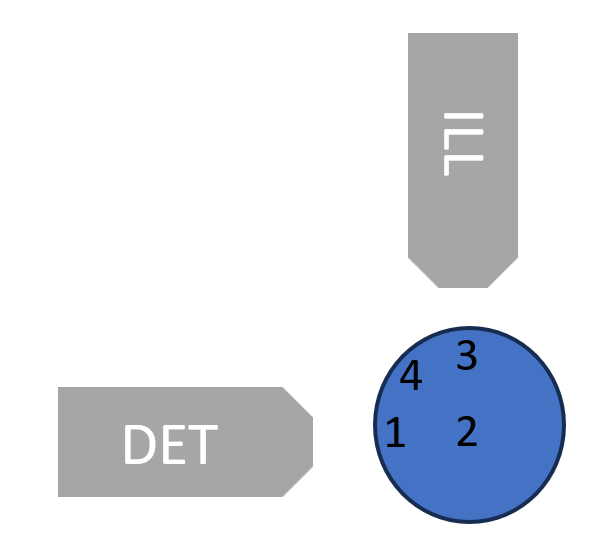
\includegraphics[width = .5\textwidth]{Bilder/Setup/sites.png}
    \caption{View from above of the measured sites. The cylindrical probe is displayed in blue, the illumination objective (ILL) and detection objective (DET) in grey.}
    \label{fig:sites}
\end{figure}

\subsection*{DDM measurements}
The bead agarose solution for the DDM measurement was prepared as before but instead of pipetting it in a topless syringe, it was injected in a thin, flexible tube which was mounted in the SPIM chamber. Measurements were taken for no pinhole, half opened pinhole and closed pinhole each in five different setups of binning and region of interest (ROI) size. Exposure time was fixed to \SI{1}{\milli\second} for all setups. $I_L$ and gain were adjusted appropriately to ensure a sufficient fluorescence intensity without saturating the camera. Each measurement consisted of a time series of \num{4000} images with the smallest possible time distance $\Delta t$ between them which was calculated for each setup by the measuring program. The setups and corresponding $\Delta t$ are listed in tab.~\ref{tab:setups}. For each combination of the five setups and the three pinhole configurations five measurements were made. 

\begin{table}
    \centering
    \begin{tabular}{c c c}
        \toprule
        binning & ROI size / px & $\Delta t$ / \si{\milli\second} \\
        \midrule
        none & 256x256 & 22 \\
        none & 128x128 & 17 \\
        2x2 & 128x128 & 12 \\
        2x2 & 64x64 & 9 \\
        4x4 & 64x64 & 8 \\
        \bottomrule
    \end{tabular}
    \caption{Binning and ROI size setups used for the measurements and corresponding time interval between the t-stack images.}
    \label{tab:setups}
\end{table}